\section{Introduction}

The ability to model and utilize long contexts has become a fundamental desired capability of modern Large Language Models (LLMs)~\cite{brown2020language,achiam2023gpt}. Consequently, scaling the context window has emerged as a key research frontier, underpinning a wide range of long-context applications such as long-horizon agentic tasks, complex reasoning, and large-scale information integration.
Despite recent progress~\cite{liu2024ringattention}, scaling context windows remains challenging for full attention due to its quadratic complexity, poor length extrapolation performance, and  KV cache cost that grows with the context length.

\begin{wrapfigure}{r}{0.42\textwidth}
\vspace{-6mm}
 \centering
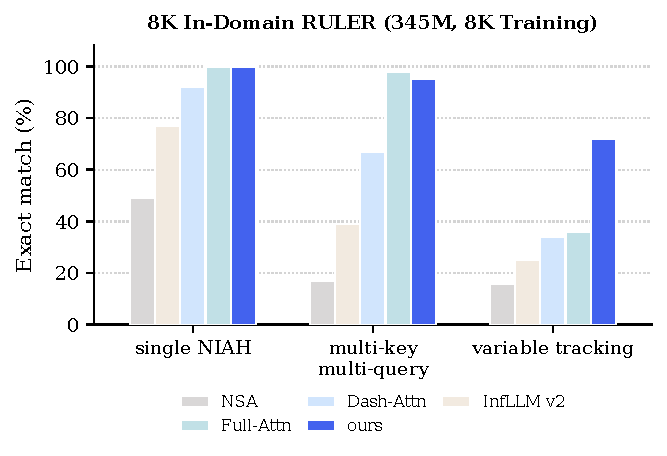
\includegraphics[trim=0 0 0 0, clip, width=0.42\textwidth]{data/ruler_8k_indomain.pdf}
\captionsetup{font=small}
\caption{In-context retrieval results.}
\label{fig:ruler_results}
\vspace{-6mm}
\end{wrapfigure}
Recently, chunk-wise sparse attention methods~\cite{hu2025efficient,yuan-etal-2025-native,DBLP:journals/corr/abs-2502-13189,huang2026nosanativeoffloadablesparse} provide a promising alternative. They selectively attend to relevant context chunks to maintain a constant computational cost, while dynamically swapping the corresponding KV caches into fast memory on demand to prevent memory explosion.
Despite their recent progress, no existing chunk-wise native sparse attention methods have achieved performance on par with full attention methods. While the performance gap may appear small for large-scale models on short-context tasks, it becomes pronounced in longer-context settings that demand precise in-context retrieval. This limitation is clearly exposed in parameter-constrained models, as evidenced by the substantial long-context retrieval gap in Fig.~\ref{fig:ruler_results}.
We argue that inaccurate chunk selection is the core challenge, which stems from weak chunk summaries and the lack of end-to-end optimization of the selection process. The nonparametric chunk summaries such as mean-pooling, have limited expressiveness and may lose crucial information.  
Although parametric summaries could be more expressive, existing methods use them only to score chunks for selection: after the hard top-$K$ chunk IDs are chosen, the summaries and chunk scores are discarded.
Consequently, the language-modeling (LM) loss cannot directly optimize the summaries or selection scores to suppress irrelevant chunks and promote chunks more useful for next-token prediction, leading to inaccurate chunk selection.


This observation motivates two desiderata: chunk summaries should be trainable end-to-end with the LM loss, and expressive enough to capture the chunk-level importance induced by full attention.
To explore this, we start from the naive Block Sparse Attention (BSA), which computes full attention, aggregates token-level attention mass within each chunk, and selects the top-$K$ chunks with the largest mass. 
Although naive BSA requires full attention computation and offers no computational savings, it yields a full-attention-derived chunk selection pattern. We use this pattern as a starting point to derive \textbf{HiLS}-Attention, an end-to-end learnable sparse attention mechanism with sufficient expressiveness to capture such chunk-level mass.
First, to estimate chunk mass without computing full attention, we append a special \textit{landmark token}~\cite{mohtashami2023random} to each chunk, from which we derive an expressive \textit{chunk summary key}. The query-summary-key scoring operation follows the first-order Taylor expansion of the full-attention induced chunk mass, thereby forming a learnable chunk-mass surrogate.
Second, HiLS makes this retrieval process end-to-end learnable by using the surrogate scores as part of the forward attention weights, via the hierarchical factorization illustrated in Fig.~\ref{fig:HilS-Attn}.
In this factorization, attention mass is first allocated across retrieved chunks and then distributed among tokens within each chunk. This avoids the quadratic full-attention pass required by naive BSA, thereby substantially reducing the computational cost during both training and inference. As a result, block selection becomes end-to-end learnable under the LM objective, allowing HiLS to assign higher scores to chunks that are more useful for prediction and suppress irrelevant ones.


To validate HiLS-Attention's alignment with naive BSA and full attention, and more importantly, assess its performance for long-context modeling, we conduct comprehensive experiments across model scales from 345M to 7B parameters, covering perplexity evaluation, short-context benchmarks, and long-context benchmarks. 
At the 345M scale, HiLS-Attention achieves comparable perplexity to full attention and better in-domain RULER~\cite{hsieh2024ruler} performance. Remarkably, despite   pretrained with only  8K context length, it extrapolates to 4M context length while maintaining over 90\% accuracy on needle-in-a-haystack retrieval, corresponding to a $512\times$ length extrapolation.
We further find that the advantage of HiLS-Attention becomes more pronounced with  256K training context length. On a challenging variable-tracking task, it improves over full attention by up to 50\%. At the 7B scale, we can convert a full-attention model to HiLS-Attention with only 50B tokens of continual training, preserving short-context performance while substantially outperforming full-attention baselines on LongBench~\cite{bai2024longbench} and exceeding the YaRN-extended~\cite{peng2024yarn} base model.
These results suggest that \textit{HiLS-Attention can not only match but also surpass these baselines in multiple settings.} 

To our best knowledge, our work is the first to provide strong empirical evidence that native sparse attention can achieve both superior long-context performance and more efficient long-context inference. Together, its strong in-domain performance, superior length extrapolation, and efficient long-context inference position HiLS-Attention as a promising alternative to full attention and a core building block for future ultra-long context modeling. 

In summary, our key contributions are as follows:
\begin{itemize}[leftmargin=*,itemsep=0.2em,topsep=0.3em]
\item We propose {HiLS-Attention}, a native sparse attention mechanism based on a hierarchical softmax, enabling end-to-end trainable sparse retrieval.
\item We connect HiLS-Attention to naive BSA from an expressiveness perspective, showing that an effective chunk summary should be mathematically aligned with the first-order Taylor expansion of the full-attention-induced chunk mass, thereby providing sufficient representational capacity for accurate block selection.
\item Our extensive experiments show that full-attention models can be cost-effectively converted to HiLS-Attention, preserving short-context performance while surpassing full attention in both in-domain long-context tasks and ultra-long-context extrapolation.
\end{itemize}

\begin{figure}[tb!]
    \centering
    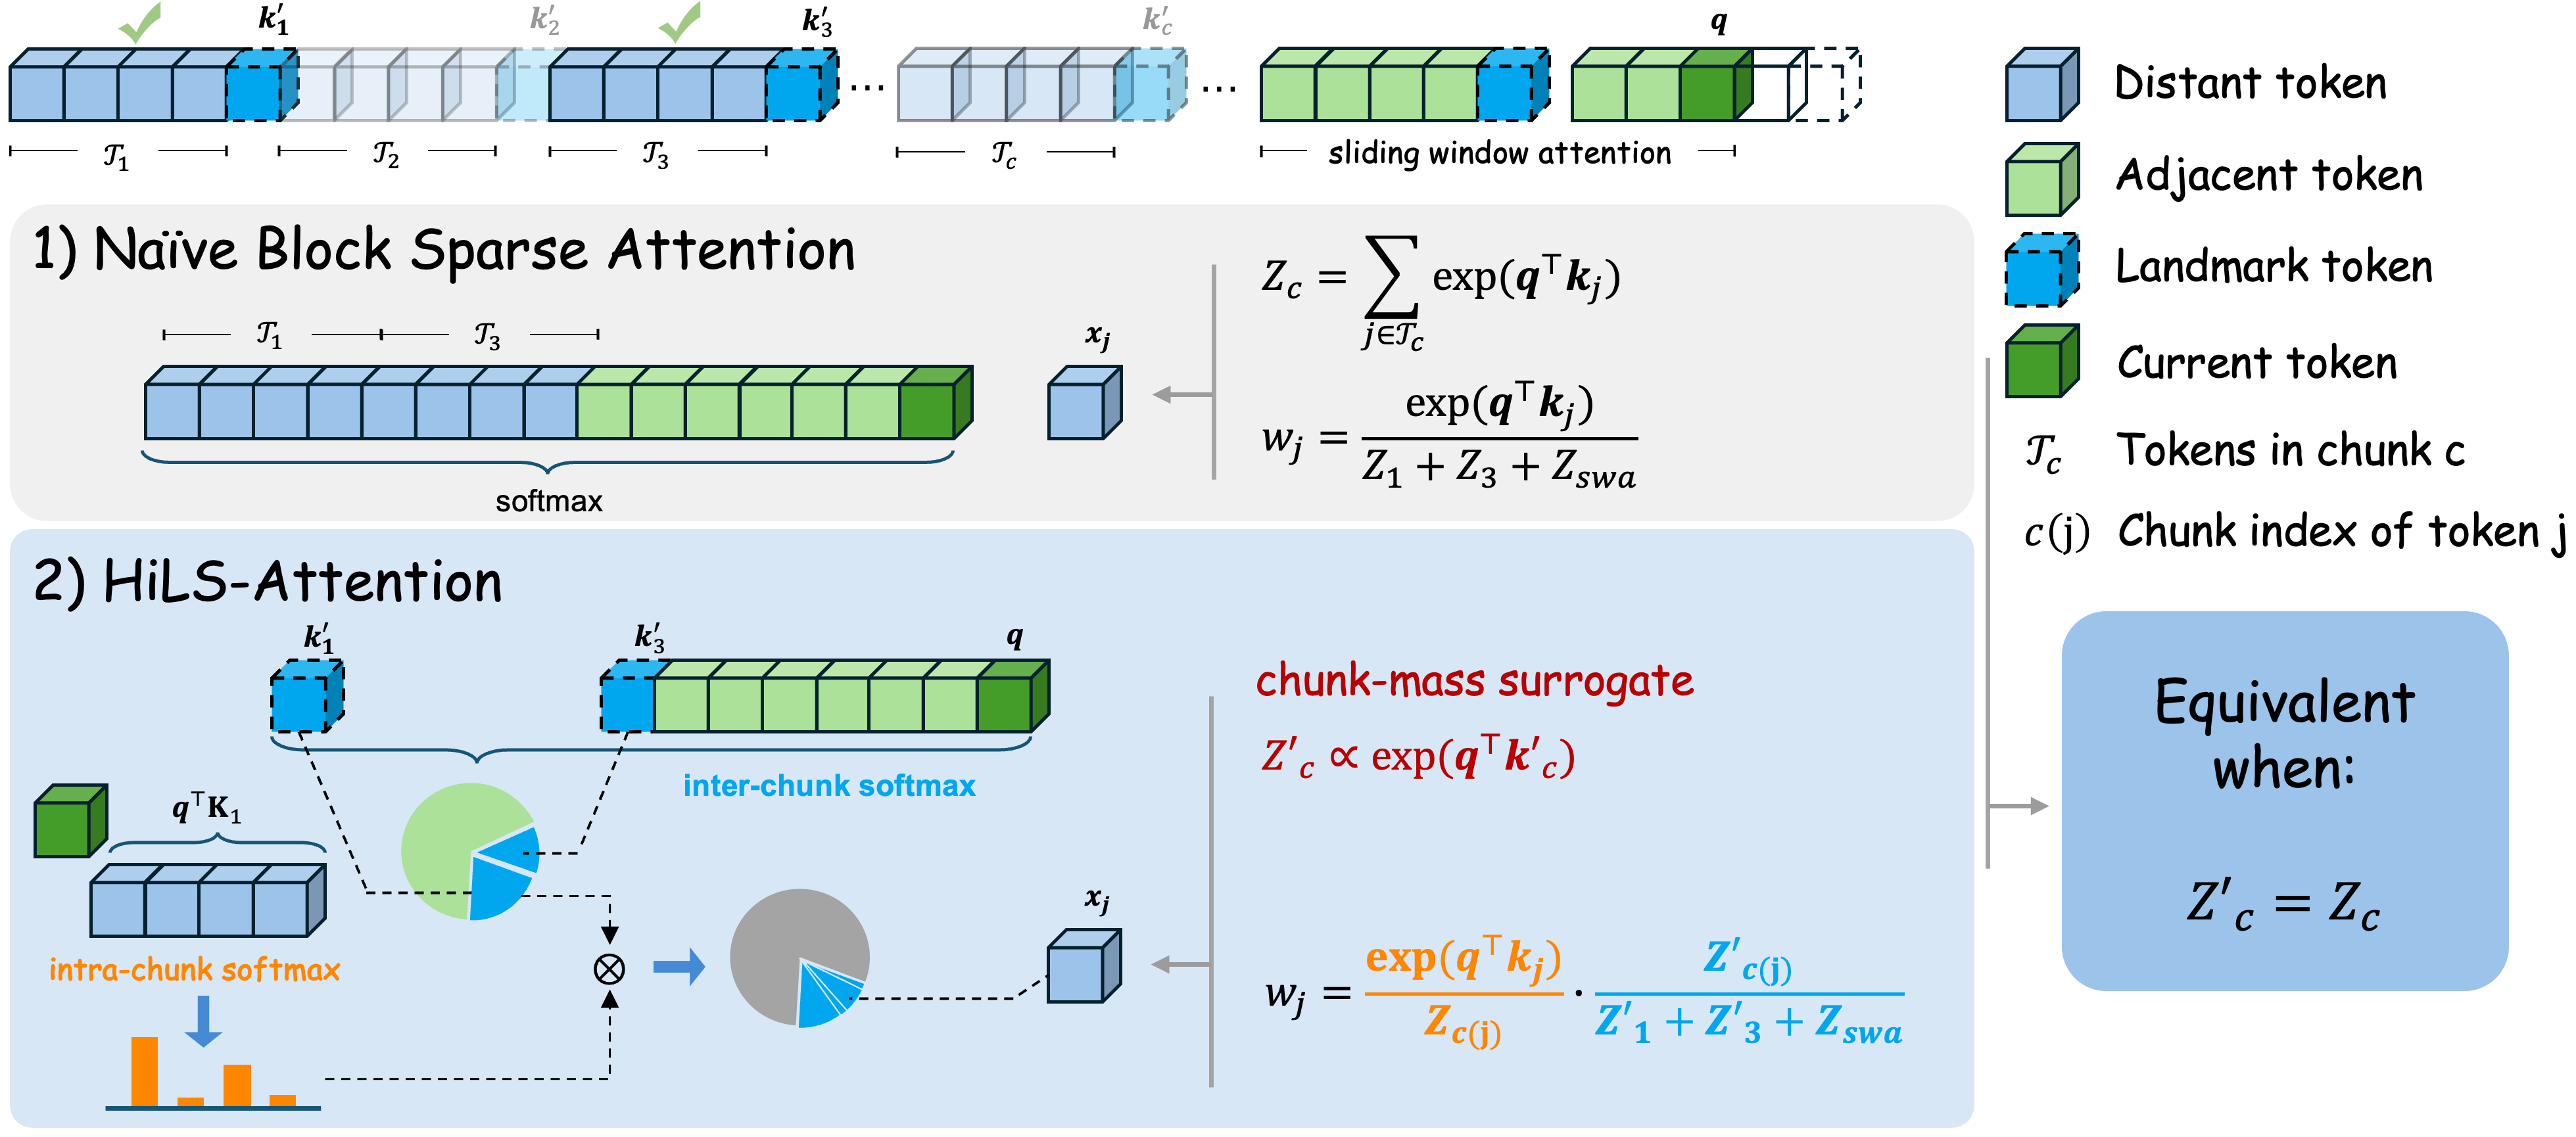
\includegraphics[width=0.98\linewidth]{data/HiLS-Attn.png}
    \caption{An overview of HiLS-Attention.
    We omit the scaling factor $\frac{1}{\sqrt{d}}$ for simplicity. Naive block sparse attention selects the top-$K$ chunks by their exact mass $Z_c$, e.g., chunks 1 and 3 when $K=2$, but computing all $Z_c$ requires a full QK computation. HiLS-Attention instead uses compressed chunk keys $k'_c$ to efficiently estimate a chunk-mass surrogate $Z'_c\propto \exp(q^\top k'_c)$. It factorizes attention into two stages: an \textbf{inter-chunk softmax}, which specifies the total attention mass assigned to each chunk, and an \textbf{intra-chunk softmax}, which distributes each chunk’s attention mass among its tokens. Since $Z'_c$ parameterizes the forward attention weights, gradients from the next-token prediction loss can be directly backpropagated to the compressed key $k'_c$, enabling end-to-end learning.}
    \label{fig:HilS-Attn}
\end{figure}
